\documentclass[11pt]{article}

\usepackage[utf8]{inputenc}
\usepackage{acl2015}
%\usepackage{times}
\usepackage{url}
%\usepackage{latexsym}
\usepackage{natbib}
\usepackage{graphicx}
\usepackage{multicol}
\usepackage{hyperref}

\title{This Time With Feeling: Sentiment to ML Headlines}

\author{Ben Arnoldy \\
  University of California, Berkeley \\
  {\tt arnoldyb@berkeley.edu} \\\And
  Mark Paluta \\
  University of California, Berkeley \\
  {\tt mpaluta@berkeley.edu} \\}
  
\date{July 2019}

\begin{document}

\maketitle

\begin{abstract}
    
\end{abstract}

\section{Introduction}
The art of good headline writing is not as simple as summarizing relevant details; it requires wit, originality, and a tone that matches the piece. Algorithms have made improvements in summarization, but still struggle with these more nuanced elements. Despite this shortcoming, algorithms could still be useful to an editor, suggesting a number of possible headlines to provide inspiration or for the editor to refine and synthesize into a final product. We propose an incremental improvement in automatic headline generation by incorporating tonal bias to match the underlying content.

\section{Background}
Headline generation is primarily approached as a single-document summarization task. The nature of headlines makes them relatively more difficult to produce with machine learning than more traditional document summaries. First, headlines tend to be shorter than the average sentence, requiring greater concision than typical ML summaries of one or more sentences. Additionally, they are often written in a short-hand style different from the body text, making extractive summarization theoretically less suitable than the more challenging task of abstractive summarization. 

Current methods of summarization involve an encoder-decoder architecture \citep{rush2015neural} with a ROUGE evaluation metric \cite{Ayana2017}. ROUGE is a recall-oriented metric to score a generated summary against a reference summary \cite{lin-2004-rouge}. Specific variants include ROUGE-N, scoring the number of common N-grams, and ROUGE-L, scoring the longest common subsequence. Recent refinements to headline generation include adversarial reward systems to combat repetition \cite{DBLP:journals/corr/abs-1902-07110} and applying state-of-the-art Transformer algorithms \cite{DBLP:journals/corr/abs-1901-07786}.

While most work on headline generation focuses exclusively on summarization, two recent papers in other summarization domains explored efforts to add desired sentiment. [Might be worth a brief background on sentiment analysis here if space allows.] One naive approach pre-processed sentences in the body of the corpus to generate sentence-level sentiment scores and simply dropped those sentences that were mismatched from the desired polarity (positive or negative) \cite{DBLP:journals/corr/abs-1802-09426}. Another more elaborate approach for customer review summaries added a discriminator to evaluate the sentiment of generated summaries, looping back to the generator to optimize on this additional criterion \cite{DBLP:journals/corr/HuYLSX17}. 

\section{Methodology}
We build a Transformer architecture, basing our algorithm off of that of Gavrilov et al \cite{DBLP:journals/corr/abs-1901-07786}, but adding sentiment into the model in the spirit of \cite{DBLP:journals/corr/abs-1802-09426} and \cite{DBLP:journals/corr/HuYLSX17}. We use sentiment-based preprocessing to upsample examples where sentiment matches well between body and headline and downsample those where the match is poor. Our objective is to increase the sentiment match between an article's headline and body while simultaneously obtaining similar ROUGE scores.

We use an encoder-decoder architecture, AdamW optimizer, and the set of specific hyperparameters outlined by Gavrilov et al \cite{DBLP:journals/corr/abs-1901-07786} as our baseline. Noteworthy parameters are listed in Table \ref{table:1}.
 
\begin{table}[h!]
\centering
\begin{tabular}{|c | c|} 
 \hline
 Hyperparameter & Value \\ [0.5ex] 
 \hline
 Hidden layer size & 1024 \\ 
 Filter size & 4096 \\
 Heads of attention & 8 \\
 Layer preprocess sequence & None \\
 Layer postprocess sequence & dropout \\
 & $\rightarrow$ add $\rightarrow$ \\
 & normalize \\
 Postprocess dropout & 0.3 \\
 Encoder layers & 4 \\
 Decoder layers & 4 \\
 Learning rate warmup steps & 4000 \\ [1ex]
 \hline
\end{tabular}
\caption{Noteworthy Hyperparameters}
\label{table:1}
\end{table}

We use a positive-negative polarity function as most research on sentiment is a simple positive-negative scale and we wish to leverage existing work. We use the \href{https://catalog.ldc.upenn.edu/LDC2008T19}{New York Times annotated corpus} to match Gavrilov et al. 
To test the quality of generated headlines, we employ the same variants on the ROUGE metric as Gavrilov et al for effective comparison of results.

Discuss post-decoder scoring of sentiment.

Specifically, we chose to work with the package \href{https://github.com/tensorflow/tensor2tensor}{\texttt{tensor2tensor}}. This package was developed by the Google Brain team and is designed for furthering research on a variety of natural language processing problems. We began by replicating the CNN/Daily Mail text summarization problem. We then adapted the architecture to accommodate a new problem of summarization, specifically headline generation rather than key point summarization, on the New York Times annotated corpus. The specific adaptations we had to make were as follows:

\begin{itemize}
    \item Prepare New York Times corpus for \texttt{tensor2tensor} ingestion by extracting filepath, headline, body, lede, word count, and other metadata, writing this data to a lot file, and performing a random train/dev/test split
    \item Define problem \texttt{Gavrilov} inheriting \texttt{Text2TextProblem}
    \item Apply a subword tokenizer to imitate Gavrilov et al's BPE tokenization
    \item Override a variety of default Universal Transformer hyperparameters as defined in Table \ref{table:1}
    \item Create optional sentiment pre-processing step
    \item Create optional random down-sampling step for control
\end{itemize}

\section{Results}
\subsection{Subsection template if needed}
\section{Discussion}
\section{Conclusion}

\begin{figure}[h!]
\centering
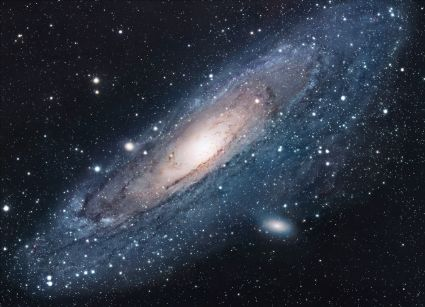
\includegraphics[scale=1.7]{universe}
\caption{The Universe}
\label{fig:universe}
\end{figure}

URL example
\url{http://acl2015.org/publication.html}.

"citing Rush here" \citep{rush2015neural}
"citing Ayana here" \cite{Ayana2017}
"citing Peng Xu here" \cite{DBLP:journals/corr/abs-1902-07110}
"citing Gavrilov here" \cite{DBLP:journals/corr/abs-1901-07786}
"citing Chaudari here" \cite{DBLP:journals/corr/abs-1802-09426}
"citing Zhiting Hu here" \cite{DBLP:journals/corr/HuYLSX17}
"citing Lin here" \cite{lin-2004-rouge}
"citing Attention is all you Need here" \cite{DBLP:journals/corr/VaswaniSPUJGKP17}

\bibliographystyle{plain}
\bibliography{references}
\end{document}




